% STATUS: Complete & Checked
Several key elements of a storage network were identified and different design decisions based around these elements have been considered. 
		
		\subsubsection{Network Connectivity}
			In order to join the network, a node must have some knowledge of where to find other nodes. This can be achieved through the use of some central authority that holds a list of nodes, enabling anyone to acquire the knowledge to use the network, or each node can act as a part of a decentralised directory, where as long as one node can be connected to, the remaining participants of the network can be discovered.
			
			Neither solution is without issues: the central authority could reduce security by providing a more important class of node that could be seen as a target by an adversary, thereby reducing the security, while the acquisition of the knowledge needed to connect to the initial node would have to occur out-of-band and any information from a decentralised directory may be subject to abuse as an element of trust is required.
			
			Although the initial connection node may seem to be much the same as the central authority, it would be possible to have several of these initial connection nodes, and as long as they are members of the network, this should be acceptable. This presents any application the freedom to use any node as an initial connection nodes, as opposed to limiting it to a single central authority.
			
			% ISSUES: This may be better suited in the API design section
			As the introduction of a central authority presents too much risk and lowers the amount of freedom compared to a distributed directory, the API should provide a mechanism to allow users of the API to set initial connection nodes in order to discover the rest of the network.
			
			Alternatively, if all users have access to some information stream where steganography could be used, it may be possible to use this for the purpose of advertising nodes. The Bitcoin Message Service uses a similar mechanism for the distribution of messages in the Bitcoin blockchain \cite{btcmsg}. As all Tor users have access to Tor directory nodes, it was hoped that hidden service descriptors could be used for steganography, however, due to the nature of Tor's directory nodes, this method is very unreliable, although possible, as some malicious nodes have used this mechanism to harvest hidden service descriptors \cite{crawl}.
			
			% Complete & Checked
			Given the nature of anonymous services, such as Tor's hidden services, the initiator of a connection is aware of the destination network identifier (or, pseudoidentity), as this is required to make the connection, although the target of the connection has no knowledge of the initiator's psuedoidentity. This has the result that connections can be considered unidirectional, although the transfer of data is bidirectional once the connection is established. In some cases, determining the pseudoidentity of the initator is desired and so this presents an interesting challenge. The initator could tell the target their pseudoidentity, which the target could either check in some way, or trust. Alternatively, as the pseudoidentity is likely to have asymmetric key backing, a digital signature could be appended to a message, proving the pseudoidentity of the initator.
			
			\begin{equation} \label{eq:internodalconnections}
\Bigg(\prod_{i=0}^{n}\bigg(1 - \frac{1}{N-1-i}\bigg)\Bigg)^{N-1}
\end{equation}

\begin{figure}[h!]
	\begin{center}
		\begin{tikzpicture}
		\begin{semilogyaxis}[
			compat=1.3,
			width=0.8\linewidth, % Scale the plot to \linewidth
			height=0.6\linewidth,
			grid=major, % Display a grid
			grid style={dashed,gray!30}, % Set the style
			xlabel=Number of nodes in network,
			ylabel=Probability,
			xmin=0, xmax=3000, xtick={0,500,1000,1500,2000,2500,3000}
		]
		\addplot[blue] 
		table[x=column 1,y=column 2,col sep=comma] {inc-data.csv}; 
		\end{semilogyaxis}
		\end{tikzpicture}
		\caption{Probability of a node not being selected by any node for inter-nodal communications}
		\label{fig:internodalconnections}
	\end{center}
\end{figure}
			
			% Complete & Checked
			The topology of the network describes how nodes organise themselves and connect to each other. In some networks, such as Freenet, nodes organise themselves into a small-world topology, where any node can communicate with any other node through some number of other nodes. This is done as a mechanism for implementing anonymity, but creates an attack vector where an adversary may be able to manipulate the topology to allow for attacks. As an existing anonymity layer will be used, there is no need to use the topology to keep nodes anonymous. Rather, it will be considered mainly for purpose of information distribution.
			
			% Complete & Checked
			Since any topology that allows node connections to be directly manipulated presents a potential attack vector, a purely logical topology, where nodes each decide who they connect to unidirectionally should be used. Since this method relies on no external influence to any node, there is a chance that some nodes may not be selected for a connection by any other node, thereby excluding them. While this is only an issue if a large number of nodes are not selected, as this effectively reduces the potential resources in the network, this number should be kept to a minimum. Formula \ref{eq:internodalconnections} shows the probability of any node not being selected by any other for a unidirectional connection. Figure \ref{fig:internodalconnections} shows this probability where each node maintains 20 unidirectional connections out. As shown, this probability is very low and even when the network is large, under the condition of periodic connection renewal, so that newer nodes are included, it is likely that all nodes will always be selected for a connection. Figure \ref{fig:internodalexample} shows an example network with the internodal connections.
			
			\begin{figure}
				\centering
				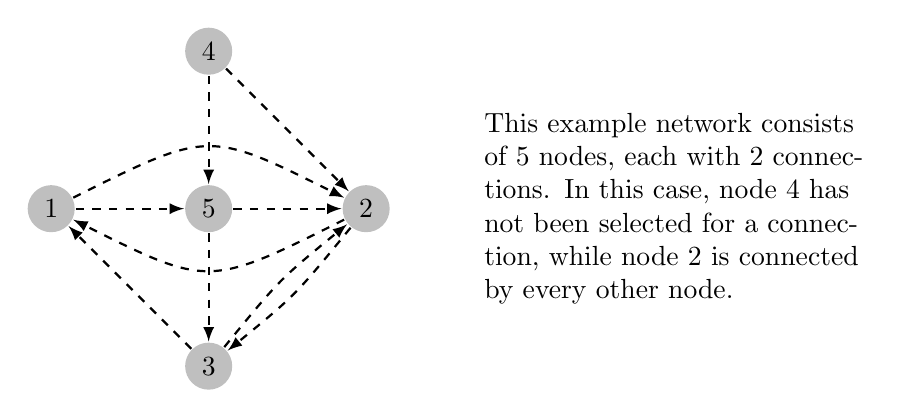
\begin{tikzpicture}[auto, thick]
				\tikzstyle{vertex}=[circle,fill=black!25,minimum size=17pt,inner sep=0pt]
				\node[vertex] (Node-1) at (-2,0) {$1$};
				\node[vertex] (Node-2) at (2,0) {$2$};
				\node[vertex] (Node-3) at (0,-2) {$3$};
				\node[vertex] (Node-4) at (0,2) {$4$};
				\node[vertex] (Node-5) at (0,0) {$5$};
				
				\draw[-latex, thick, dashed, black] (Node-1) .. controls (0,1) .. (Node-2);
				\draw[-latex, thick, dashed, black] (Node-1) -- (Node-5);
				
				\draw[-latex, thick, dashed, black] (Node-2) .. controls (0,-1) .. (Node-1);
				\draw[-latex, thick, dashed, black] (Node-2) .. controls (1.1,-1.1) .. (Node-3);
				
				\draw[-latex, thick, dashed, black] (Node-3) .. controls (0.9,-0.9) .. (Node-2);
				\draw[-latex, thick, dashed, black] (Node-3) -- (Node-1);
				
				\draw[-latex, thick, dashed, black] (Node-4) -- (Node-2);
				\draw[-latex, thick, dashed, black] (Node-4) -- (Node-5);
				
				\draw[-latex, thick, dashed, black] (Node-5) -- (Node-3);
				\draw[-latex, thick, dashed, black] (Node-5) -- (Node-2);
				
				\node[text width=5cm] at (6,0) {This example network consists of 5 nodes, each with 2 connections. In this case, node 4 has not been selected for a connection, while node 2 is connected by every other node.};
				
				%\draw[-latex, thick, dashed, black] (Node-2) -- (Node-1);
				\end{tikzpicture}	
				
				\caption{High-level internodal connection diagram example}
				\label{fig:internodalexample}
				%\end{center}
			\end{figure}
			
			
			
			
			
		\subsubsection{Packet Classes}
			\begin{description}[topsep=-5pt,itemsep=-1ex,partopsep=2ex,parsep=1.5ex]
				\item[Data as Notifications] \hfill \\
				A single class of data packet is used, where the intended message and notification of the existence of said message are combined. This means that if a notification is successful, the data will always be available, resulting in lower delivery latency. However, as the size of some packets could be large, and the majority of this information is destined for most nodes, this is likely to be wasteful and could cause scalability issues.
				\item[Notifications Referencing Data] \hfill \\
				Two classes of packet are used: a data packet that is just for storing data and a notification packet that is only for notifying a node about the existence of a data packet. While all nodes still need to check all the notifications, only a subset of all nodes need to be in possession of the data packets. In addition, the notifications may also include information such as some known locations of the desired data packet (rendezvous nodes). This method has the potential to reduce the availability of data packets that are not distributed well throughout the network.
				\item[Notifications with Small Payload] \hfill \\
				Each notification packet is a union\footnote{A union type is one that provides an either-or contents structure.} of a small payload or a data packet reference. The total size of this is still comparable to that of a typical notification packet. The result of this structure would be very high availability for any small payload.
			\end{description}
			Given that notifications with small payloads have the potential to provide maximal flexibility while also reducing the load on the network, these will be used.
			
		\subsubsection{Information Distribution and Delivery}
			Distributing the information across the network must occur in order to keep the availability of information high. In order to receive a message, everyone must either check every message, or there must be some form of delegation to a third party, or parties, that must perform the same role.
			
			Systems, such as Bitmessage, take the approach that everyone can attempt to determine if a message is for them, whereas other systems, such as email, take advantage that the recipient of a message can be determined and use this to place the message in a predictable location. Other networks, such as Freenet, move the obligation of notification to out-of-band communications, meaning they do not address this issue.
			
			As the Bitmessage network grows, it splits into ``streams''~\cite{bitmsg}, effectively creating smaller subnetworks. Membership of a stream can be a function of some identifying element of the user, such as a public key (figure \ref{fig:stream-normal}). Although this method is promising in terms of scalability, it has some disadvantages for the anonymity of the network. This type of optimisation is only possible where each stream has enough members such that if the stream was isolated, the property of anonymity would hold. Under the assumption that one user controls exactly one node, it is enough for the node membership under any stream for be sufficiently high. However, if this assumption cannot be made, then it opens the possibility to deanonymisation attacks. The worst-case for this attack is that it may be possible to determine the public key, and therefore the identity that a node is interested in retrieving messages for. This would occur where an adversary is able to isolate a node in a stream (figure \ref{fig:stream-malicious}) and could happen where an adversary creates a large number of nodes with similar public keys (through trial and error, or otherwise) to the target node. Although this may only reveal the recipient's identity for new packets in the stream where the isolation attack is taking place, it is still undesirable.
			
			% Diagrams produced from modified code originally made by andrino Claudio 2011 - http://claudiofiandrino.altervista.org/

\definecolor{pinegreen}{cmyk}{0.92,0,0.59,0.25}
\definecolor{royalblue}{cmyk}{1,0.50,0,0}
\definecolor{lavander}{cmyk}{0,0.48,0,0}
\definecolor{violet}{cmyk}{0.79,0.88,0,0}

\tikzstyle{legend_overlay}=[rectangle, rounded corners, thin,
top color= white,bottom color=white, draw=black,
minimum width=2.5cm, minimum height=0.8cm,
black,rotate=90]
\tikzstyle{legend_general}=[rectangle, rounded corners, thin,
top color=white,bottom color=white, draw=black,
minimum width=2.5cm, minimum height=0.8cm,
black]
\begin{figure}
	\centering
	\begin{tikzpicture}[auto, thick]
	\tikzstyle{vertex}=[circle,fill=black!25,minimum size=17pt,inner sep=0pt]

	\node[legend_overlay] at (-6.5,0){\textsc{Before Split}};
	\node[legend_overlay] at (-6.5,-5){\textsc{After Split}};
	
	\node[cloud, draw=black, cloud puffs=16, cloud puff arc= 100, minimum width=7cm, minimum height=4.5cm, aspect=1] (Stream-main) at (0,0) {};
	\node[legend_general] at (0,1.6){Stream for PKs 0* to f*};
	\foreach \name/\y/\pk in {a/0/PK: 0fa79\ldots, b/0.7/PK: c2955\ldots, c/1.4/PK: 3795a\ldots, d/2.1/PK: ee775\ldots} {
		\node[vertex] (A-\name) at (-1.3,0.8-\y) {$\name$};	\node[right] (A-label-a) at (-1,0.8-\y) {$\pk$};
	}
	
	\node[cloud, draw=black, cloud puffs=16, cloud puff arc= 100, minimum width=5cm, minimum height=3.5cm, aspect=1] (Stream-split1) at (-3,-5) {};
	\node[legend_general] at (-3,-3.9){{Stream for PKs 0* to 7*}};
	\foreach \name/\y/\pk in {a/0/PK: 0fa79\ldots, c/0.7/PK: 3795a\ldots} {
		\node[vertex] (B-\name) at (-4.3,-5-\y) {$\name$};	\node[right] (B-label-a) at (-4,-5-\y) {$\pk$};
	}
	
	\node[cloud, draw=black, cloud puffs=16, cloud puff arc= 100, minimum width=5cm, minimum height=3.5cm, aspect=1] (Stream-split2) at (3,-5) {};
	\node[legend_general] at (3,-3.9){{Stream for PKs 8* to f*}};
	\foreach \name/\y/\pk in {b/0/PK: c2955\ldots, d/0.7/PK: ee775\ldots} {
		\node[vertex] (C-\name) at (1.7,-5-\y) {$\name$};	\node[right] (C-label-a) at (2.0,-5-\y) {$\pk$};
	}
	
	\draw[-latex, thick, black] (Stream-main) -- (Stream-split1);
	\draw[-latex, thick, black] (Stream-main) -- (Stream-split2);
	\end{tikzpicture}
	\caption{Example of intended stream usage}
	\label{fig:stream-normal}
%	\end{center}
\end{figure}


\begin{figure}
	\centering
	\begin{tikzpicture}[auto, thick]
	\tikzstyle{vertex}=[circle,fill=black!25,minimum size=17pt,inner sep=0pt]
	
	\node[cloud, fill=white, draw=black, cloud puffs=16, cloud puff arc= 100, minimum width=7cm, minimum height=4.5cm, aspect=1] at (0,0) {};
	\node[legend_general] at (0,1.6){{Stream for PKs 0fa*}};
	
	\foreach \name/\y/\pk in {E/0/PK: 0fa73\ldots, F/0.7/PK: 0fa18\ldots, H/2.1/PK: 0fa9c\ldots} {
		\node[vertex, fill=black!70!white, text=white] (A-\name) at (-1.3,0.8-\y) {$\name$};
		\node[right, text=black] (A-label-a) at (-1,0.77-\y) {$\pk$};
	}
	
	\foreach \name/\y/\pk in {g/1.4/PK: 0faf2\ldots} {
		\node[vertex] (A-\name) at (-1.3,0.8-\y) {$\name$};
		\node[right] (A-label-a) at (-1,0.8-\y) {$\pk$};
	}
	\end{tikzpicture}
	\caption{Example of malicious nodes isolating a legitimate node}
	\label{fig:stream-malicious}
	%\end{center}
\end{figure}


%\begin{figure}
%	\centering
%	\begin{tikzpicture}[auto, thick]
%	\tikzstyle{vertex}=[circle,fill=black!25,minimum size=17pt,inner sep=0pt]
%		\node[vertex] (Node-1) at (-2,0) {$1$};
%		\node[vertex] (Node-2) at (2,1.5) {$2$};
%		\node[vertex] (Node-3) at (2,0) {$3$};
%		\node[vertex] (Node-4) at (2,-1.5) {$4$};
%		
%		\node[vertex] (Node-X) at (5,2) {$X$};
%		\node[right] (Node-label-X) at (5.5,2) {Node X};
%		
%	\tikzstyle{vertex}=[circle,fill=yellow!25,draw=black,minimum size=12pt,inner sep=0pt]
%		
%		\node[vertex] (Packet-y) at (5,1.2) {$y$};
%		\node[right] (Packet-label-y) at (5.5,1.2) {Packet y};
%	
%		\node[vertex] (Packet-1-a) at (-2.5,0.5) {$a$};
%		\node[vertex] (Packet-1-b) at (-2.7,0) {$b$};
%		%\node[vertex] (Packet-1-c) at (-2.5,-0.5) {$c$};
%		\draw[thick, black] (Node-1) -- (Packet-1-a);
%		\draw[thick, black] (Node-1) -- (Packet-1-b);
%		%\draw[thick, black] (Node-1) -- (Packet-1-c);
%		
%		\node[vertex] (Packet-2-a) at (2.5,2) {$a$};
%		\node[vertex] (Packet-2-b) at (2.7,1.5) {$b$};
%		\draw[thick, black] (Node-2) -- (Packet-2-a);
%		\draw[thick, black] (Node-2) -- (Packet-2-b);
%		
%		\node[vertex] (Packet-3-a) at (2.5,0.5) {$a$};
%		\node[vertex] (Packet-3-c) at (2.7,0) {$c$};
%		\draw[thick, black] (Node-3) -- (Packet-3-a);
%		\draw[thick, black] (Node-3) -- (Packet-3-c);
%		
%		\node[vertex] (Packet-4-b) at (2.5,-1) {$b$};
%		\node[vertex] (Packet-4-d) at (2.7,-1.5) {$d$};
%		\draw[thick, black] (Node-4) -- (Packet-4-b);
%		\draw[thick, black] (Node-4) -- (Packet-4-d);
%		
%		\node[text width=5cm] at (6,-1) {Node 1 selects nodes 2 and 3 to be its connections into the network};
%		
%		\draw[-latex, thick, dashed, black] (4.5,0.4) -- (5.4,0.4);
%		\node[right] (Arrow) at (5.5,0.4) {Connection};
%		
%		\draw[-latex, thick, dashed, black] (Node-1) -- (Node-2);
%		\draw[-latex, thick, dashed, black] (Node-1) -- (Node-3);
%		%\node[right] (A-label-a) at (-1,0.8-\y) {$\pk$};
%	\end{tikzpicture}	
%	
%	\vspace*{0.1cm} \hrulefill \vspace*{0.1cm}
%	
%		\begin{tikzpicture}[auto, thick]
%		\tikzstyle{vertex}=[circle,fill=black!25,minimum size=17pt,inner sep=0pt]
%		\node[vertex] (Node-1) at (-2,0) {$1$};
%		\node[vertex] (Node-2) at (2,1.5) {$2$};
%		\node[vertex] (Node-3) at (2,0) {$3$};
%		\node[vertex] (Node-4) at (2,-1.5) {$4$};
%		
%		\tikzstyle{vertex}=[circle,fill=yellow!25,draw=black,minimum size=12pt,inner sep=0pt]
%		
%		\node[vertex] (Packet-1-a) at (-2.5,0.5) {$a$};
%		\node[vertex] (Packet-1-b) at (-2.7,0) {$b$};
%		\node[vertex] (Packet-1-N) at (-2.5,-0.5) {$N$};
%		\draw[thick, black] (Node-1) -- (Packet-1-a);
%		\draw[thick, black] (Node-1) -- (Packet-1-b);
%		\draw[thick, black] (Node-1) -- (Packet-1-N);
%		
%		\node[vertex] (Packet-2-a) at (2.5,2) {$a$};
%		\node[vertex] (Packet-2-b) at (2.7,1.5) {$b$};
%		\draw[thick, black] (Node-2) -- (Packet-2-a);
%		\draw[thick, black] (Node-2) -- (Packet-2-b);
%		
%		\node[vertex] (Packet-3-a) at (2.5,0.5) {$a$};
%		\node[vertex] (Packet-3-c) at (2.7,0) {$c$};
%		\draw[thick, black] (Node-3) -- (Packet-3-a);
%		\draw[thick, black] (Node-3) -- (Packet-3-c);
%		
%		\node[vertex] (Packet-4-b) at (2.5,-1) {$b$};
%		\node[vertex] (Packet-4-d) at (2.7,-1.5) {$d$};
%		\draw[thick, black] (Node-4) -- (Packet-4-b);
%		\draw[thick, black] (Node-4) -- (Packet-4-d);
%		
%		\node[text width=5cm] at (6,0) {Node 1 inserts a new packet N into the network by forwarding it along the connections, using Nodes 2 and 3 as rendezvous points};
%		
%		\draw[thick, red] (Node-1) -- (Node-2);
%		\draw[thick, red] (Node-1) -- (Node-3);
%		
%		\draw[-latex, thick, dashed, black] (Node-1) -- (Node-2);
%		\draw[-latex, thick, dashed, black] (Node-1) -- (Node-3);
%		%\node[right] (A-label-a) at (-1,0.8-\y) {$\pk$};
%		\end{tikzpicture}
%	
%	
%	
%	\caption{TEST}
%	\label{fig:TEST}
%	%\end{center}
%\end{figure}















			
			While all nodes need to check all messages to a degree, this mechanism is only required to notify of a message. Hence, instead of combining the notification and data functionality in a single packet, and having everyone acquire all of these, a split can be made. This would still require everyone to acquire and check all the notification packets, but these notifications could point to a data packet elsewhere on the network, along with a collection of rendezvous nodes that are known to be in possession of these data packets.
			
			\subsubsection{Broadcast Handling}
			Notifications will be broadcast to at least all nodes that are members of a stream, this is likely to be the bottleneck of the system. The handling of broadcasts should therefore be subject to optimisation where possible.

			\begin{description}[topsep=-5pt,itemsep=-1ex,partopsep=2ex,parsep=1.5ex]
				\item[Universal Polling (UP)] \hfill \\
				Nodes query other nodes for a list of their stored broadcasts, acting like a distributed hash table. The querying node can then request any broadcast it does not have stored. If the rate of broadcasts inserted into the network is greater than the rate they expire, then the size of the query response will grow unsustainably.
				\item[Active Forwarding (AF)] \hfill \\
				Upon receiving a broadcast for the first time, the node forwards it onto all of its connections. This does not require any list of broadcasts to be distributed, saving on some overhead. However, as the node initiating the forwarding is unaware if the nodes are in possession of the broadcast, the receiving node will be responsible for signalling that further transfer is not required, probably in the form of terminating the connection.
				\item[Selective Polling (SP)] \hfill \\
				When a node receives a broadcast, it also stores the time of receipt. When a node polls another node, it stores the time of polling for that node. In a similar way to UP, polling is used to gather a list of broadcasts, but a parameter specifying the last time of polling is passed too. The polled node returns the list of all broadcasts that it received after this time. This has potential anonymity implications where it may reveal the time at which a node received a broadcast. However, this can be negated by having the receiving node add a small random time to the real time of receipt.
			\end{description}
			\begin{figure}
	\centering
		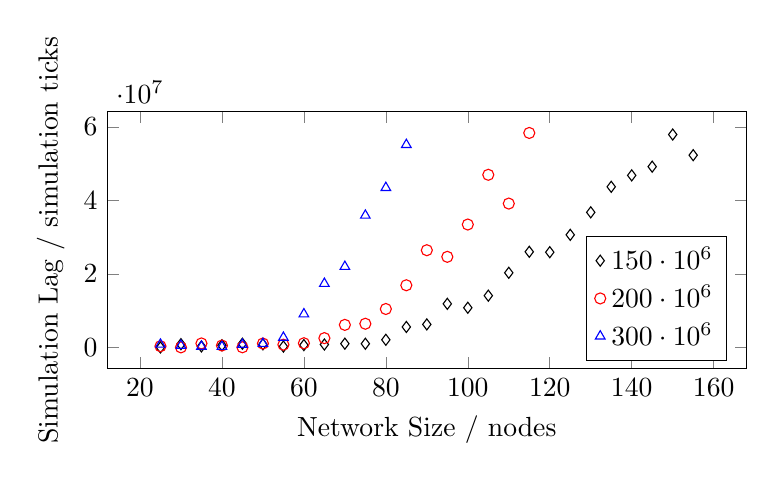
\begin{tikzpicture}
			\begin{axis}[
					width=0.8\linewidth,
					height=0.4\linewidth,
					xlabel=Network Size / nodes,
					ylabel=Simulation Lag / simulation ticks,
					legend entries={$150\cdot10^6$, $200\cdot10^6$, $300\cdot10^6$},
					legend pos=south east
				]
			%	\addlegendentry{\hspace{-.6cm}\textbf{Time}}
				\addplot[
					scatter,
					only marks,
					point meta=explicit symbolic,
					scatter/classes={
						a={mark=diamond,black},
						b={mark=o,draw=red},
						d={mark=triangle,blue}
						},
				]
				table[meta=label] {
					x y label
					25	24541 a
					30	907572 a
					35	304920 a
					40	616387 a
					45	1031117 a
					50	864221 a
					55	258485 a
					60	653754 a
					65	809943 a
					70	1048788 a
					75	1026927 a
					80	2100095 a
					90	6288081 a
					85	5590600 a
					95	11880910 a
					100	10815227 a
					105	14100952 a
					110	20324960 a
					115	26029089 a
					125	30645860 a
					120	25923148 a
					130	36772925 a
					135	43713637 a
					140	46817286 a
					150	57932035 a
					145	49191305 a
					155	52311392 a
					25	357262 b
					30	33972 b
					35	1112397 b
					40	540416 b
					45	61033 b
					50	1082894 b
					55	775513 b
					60	1163609 b
					65	2553731 b
					70	6156550 b
					75	6463167 b
					80	10478434 b
					85	16933039 b
					95	24665926 b
					90	26465847 b
					110	39154681 b
					100	33453911 b
					115	58362416 b
					105	46980354 b
					25	846698 d
					35	269968 d
					30	541413 d
					40	228635 d
					45	811461 d
					50	1057005 d
					55	2725045 d
					60	9102614 d
					65	17391255 d
					70	22003664 d
					80	43466949 d
					75	35927541 d
					85	55167398 d	
				};
			\end{axis}
		
		\end{tikzpicture}
		\caption{Simulation lag for network sizes for varying simulation lengths (UP)}
		\label{fig:simulation-lag}
	%\end{center}
%\end{figure}
	\vspace*{1cm}
%\begin{figure}
	\centering
		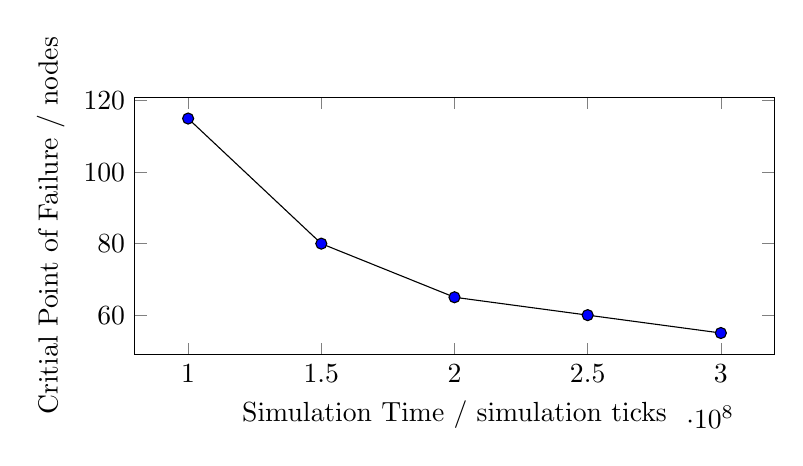
\begin{tikzpicture}
		\begin{axis}[
			width=0.8\linewidth,
			height=0.4\linewidth,
			xlabel=Simulation Time / simulation ticks,
			ylabel=Critial Point of Failure / nodes,
			xtick={100e6,150e6,200e6,250e6,300e6}
		]
		\addplot[
		scatter,
		scatter/use mapped color={draw=none, fill=blue}
		]
		table {
			x y
			100e6	115
			150e6	80
			200e6	65
			250e6	60
			300e6	55
		};
		\end{axis}
		\end{tikzpicture}
		\caption{Critical point of failure for simulation lengths (UP)}
		\label{fig:critical-point}
	%\end{center}
%\end{figure}
	\vspace*{1cm}
%\begin{figure}
	\centering
		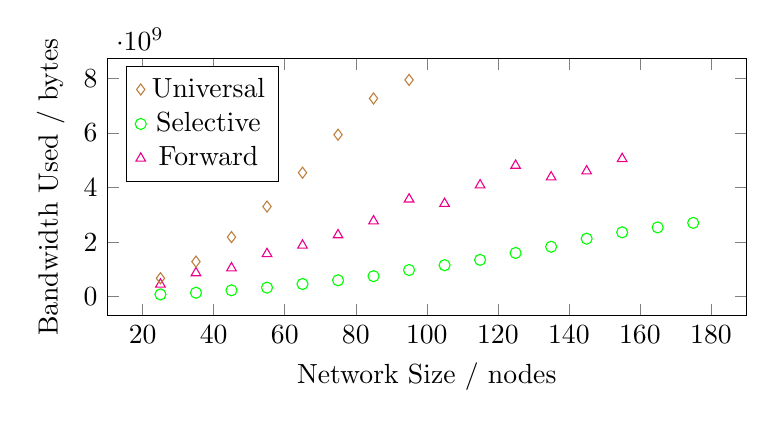
\begin{tikzpicture}
		\begin{axis}[
		width=0.8\linewidth,
		height=0.4\linewidth,
		xlabel=Network Size / nodes,
		ylabel=Bandwidth Used / bytes,
		legend entries={Universal, Selective, Forward},
		legend pos=north west
		]
		%	\addlegendentry{\hspace{-.6cm}\textbf{Time}}
		\addplot[
		scatter,
		only marks,
		point meta=explicit symbolic,
		scatter/classes={
			universal={mark=diamond,brown},
			selective={mark=o,draw=green},
			forward={mark=triangle,magenta}
		},
		]
		table[meta=label] {
			x y label
			25 456019780 forward
			35 872253165 forward
			45 1048887570 forward
			55 1573692515 forward
			65 1881124400 forward
			75 2262434505 forward
			85 2771544750 forward
			95 3573927345 forward
			105 3411036380 forward
			115 4092502880 forward
			125 4807955340 forward
			135 4384191915 forward
			145 4602090000 forward
			155 5055210185 forward

			25 677312540 universal
			35 1287235525 universal
			45 2185638925 universal
			55 3304297955 universal
			65 4545322280 universal
			75 5936811385 universal
			85 7265776430 universal
			95 7945404335 universal
			
			25 85397100 selective
			35 147088405 selective
			45 235060850 selective
			55 333573715 selective
			65 466682360 selective
			75 602788785 selective
			85 754004910 selective
			95 979054255 selective
			105 1156023540 selective
			115 1351527220 selective
			125 1604653050 selective
			135 1832297135 selective
			145 2127906425 selective
			155 2361108570 selective
			165 2540262770 selective
			175 2706737490 selective
		};
		\end{axis}
		
		\end{tikzpicture}
		\caption{Bandwidth used for different broadcast handling methods near steady-state}
		\label{fig:bandwidth-required}
\end{figure}
			Simulations for each of the 3 broadcast handling methods were run for a set period of time. For the interval up to this time, nodes are stimulated, adding tasks for them to perform, such as querying another node or pushing data into the network. After the allowed simulation time, no more stimulations occur and the remaining tasks are allowed to complete. The interval from stopping stimulations to the end of the simulation is referred to as the simulation lag. More detail on the simulator can be found in appendix \ref{simulator}. It should be noted that time, in this context, is measured in simulation ticks, not the real time the simulation takes to complete. Small simulation lag values are what is expected to result from a sustainable system where tasks do not accumulate.
			
			Simulation results are not absolute, and real scalability and performance results will be dependant on real network usage. The simulations presented here, subject to minor variation in the random nature of simulating usage, have been conducted under the same usage conditions.
			
			Running the simulation for UP for a set time, while varying the size of the network results in the graph shown in figure \ref{fig:simulation-lag}. The point where the method fails for a simulation interval of $150\cdot10^6$ ticks, can be seen to occur at 80 nodes. For UP, the points of failure for different simulation times were plotted, as shown in figure \ref{fig:critical-point}. This downward trend indicates that the number of nodes needed for network failure decreases the longer the network is active.
			
			Simulations for SP and AF were also conducted, but points of failure could not be determined.
			
			The simulations were run for $300\cdot10^6$ ticks, to achieve near steady-state behaviour in the network. The bandwidth used over each of the simulations was compared, as shown in figure \ref{fig:bandwidth-required}.
			
			SP has the potential to require the least bandwidth for broadcasts. AF may also be useful to support for the purpose of initial packet distribution, to both increase availability faster and to increase anonymity by hiding the original source of packets.
			